\documentclass[tikz,border=3pt]{standalone}
\usepackage[utf8]{inputenc}
\usepackage[T1]{fontenc}
\usepackage{lmodern}
\renewcommand{\familydefault}{\sfdefault}
\usepackage{sansmath}\sansmath
\usepackage{chemfig}
\usepackage{pgfplots}\pgfplotsset{compat=1.18,/pgf/number format/use comma,/pgf/number format/1000 sep={.}}
\usetikzlibrary{arrows.meta,calc,positioning,decorations.pathmorphing,patterns}
% paleta del sitio
\definecolor{nar}{HTML}{E8680C}\definecolor{narc}{HTML}{FFB35C}\definecolor{hielo}{HTML}{FFF3E8}
\definecolor{tinta}{HTML}{1D1D1F}\definecolor{gris}{HTML}{6E6E73}\definecolor{lila}{HTML}{7C5CF0}
\definecolor{azul}{HTML}{2F6FD6}\definecolor{menta}{HTML}{17A673}\definecolor{coral}{HTML}{E8342A}
\begin{document}
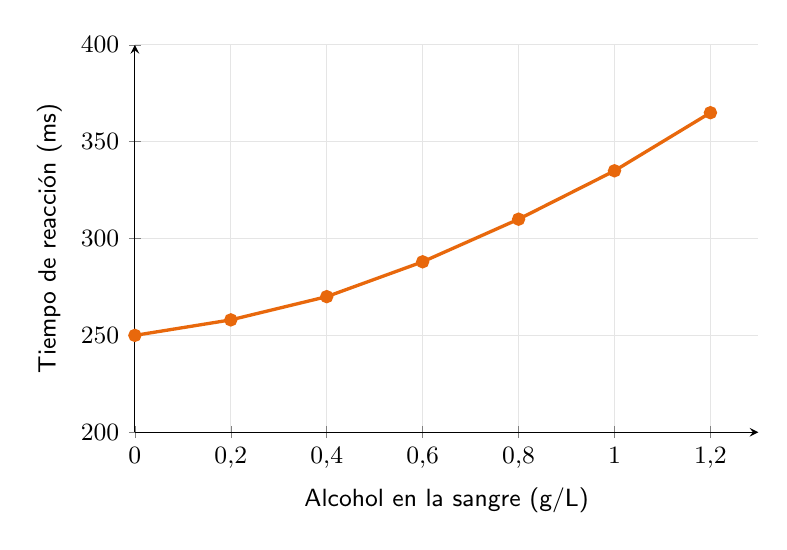
\begin{tikzpicture}[font=\small]
\begin{axis}[axis lines=left,grid=major,grid style={gray!20},xlabel={Alcohol en la sangre (g/L)},ylabel={Tiempo de reacción (ms)},
  width=9.5cm,height=6.5cm,xmin=0,xmax=1.3,ymin=200,ymax=400,xtick={0,0.2,...,1.2},ytick={200,250,...,400},
  xticklabel style={/pgf/number format/fixed,/pgf/number format/precision=1}]
\addplot[nar,very thick,mark=*,mark options={fill=nar,scale=0.9}] coordinates {(0,250)(0.2,258)(0.4,270)(0.6,288)(0.8,310)(1.0,335)(1.2,365)};
\end{axis}
\end{tikzpicture}
\end{document}
